\documentclass{article}
\usepackage{amsmath}
\usepackage{amssymb}
\usepackage{nicefrac}
\usepackage{graphicx}
\usepackage{caption}
\usepackage{prettyref}
\usepackage{float}
\newrefformat{fig}{[\ref{#1}]}

\author{Cláudio Ferreira Carneiro - RA 263796}
\title{EFC 1}
\begin{document}
    \maketitle
    \pagenumbering{gobble}
    \newpage
    \pagenumbering{arabic}
    \section[]{Atividades teóricas}
    \subsection*{Exercício 01}
    \paragraph{a)}
    \begin{align*}
        P(X=1)&=\frac{1}{8} + \frac{1}{3} =\frac{11}{24}\\
        P(Y=1)&=\frac{3}{8} + \frac{1}{3} =\frac{17}{24}\\
        P(X=0)&=\frac{1}{6} + \frac{3}{8} =\frac{13}{24}\\
        P(Y=0)&=\frac{1}{6} + \frac{1}{8} =\frac{7}{24}\\
    \end{align*}
    \paragraph{b)}
    \begin{align*}
        P(X=0|Y=0)&=\frac{\nicefrac{1}{6}}{\nicefrac{1}{6} + \nicefrac{1}{8}} \approx57,14\%
    \end{align*}
    \paragraph{c)}
    \begin{align*}
        E[X] &= \frac{1}{8} + \frac{1}{3} = \frac{11}{24}\\
        E[Y] &= \frac{3}{8} + \frac{1}{3} = \frac{17}{24}
    \end{align*}
    \paragraph{d)}
    Não são independentes. $P(X|Y)\neq P(X)$, logo a ocorrência de $X$ é afetada por $Y$.
    \begin{align*}
        P(X=1|Y=1)&=\frac{\nicefrac{1}{8}}{\nicefrac{3}{8}+\nicefrac{1}{3}}\\
        &\approx 0.1765 \neq 0.125\\
    \end{align*}
    \subsection*{Exercício 02}
    \paragraph{a)}
    \begin{align*}
        P(X=1)&=\nicefrac{3}{4}&
        P(X=0)&=\nicefrac{1}{4}&
        P(Y=0)&=\nicefrac{3}{8}&
        P(Y=1)&=\nicefrac{5}{8}
    \end{align*}
    \begin{align*}
        H(X)&=\frac{-3}{4}\log_{2}\frac{3}{4} + \frac{-1}{4}\log_{2}\frac{1}{4} 
        &\approx 0.8113\\
        H(Y)&=\frac{-3}{8}\log_{2}\frac{3}{8} +\frac{-5}{8}\log_{2}\frac{5}{8} 
        &\approx 0.9544\\
        H(X,Y)&=\frac{-1}{4}\log_{2}\frac{1}{4} + 
                \frac{-3}{8}\log_{2}\frac{3}{4} +
                \frac{-3}{8}\log_{2}\frac{3}{4}
                &\approx 1,5613
    \end{align*}
    \paragraph{b)}
    \begin{align*}
       P(Y=0|X=0)&=0 & P(Y=1|X=0)&=1 & P(Y=0|X=1)&=0.5 & P(Y=1|X=1)&=0.5 \\
       P(X=0|Y=0)&=0 & P(X=1|Y=0)&=1 & P(X=0|Y=1)&=0.4 & P(X=1|Y=1)&=0.6 
    \end{align*}
    \begin{align*}
        H(Y|X)&=\frac{-1}{4}\log_{2}1 + \frac{-3}{8}\log_{2}0.5 + \frac{-3}{8}\log_{2}0.5=0.75 \\ 
        H(X|Y)&=\frac{-1}{4}\log_{2}0.4 + \frac{-3}{8}\log_{2}1 + \frac{-3}{8}\log_{2}0.6=0.6068\\
        H(X,Y)&=H(X) + H(Y|X)=H(Y) + H(X|Y) 
    \end{align*}
    \paragraph{c)}
    \begin{align*}
        I(X,Y)&=H(X)-H(X|Y)=H(Y)-H(Y|X)\approx 0.2044  
    \end{align*}
    \subsection*{Exercício 03}
    \paragraph{a)}
    \begin{align*}
        g(x) &= g_1(x) - g_2(x)\\
        g(x)=0&=\frac{1}{\sqrt{2\pi}}e^{\frac{-1}{2}(\frac{x+1}{1})^2} - \frac{1}{\sqrt{2\pi}}e^{\frac{-1}{2}(\frac{x-1}{1})^2}\\
            0&=\frac{1}{\sqrt{2\pi}}\left(e^{\frac{-1}{2}(\frac{x+1}{1})^2} - e^{\frac{-1}{2}(\frac{x-1}{1})^2}\right)\\
           e^{\frac{-1}{2}(\frac{x+1}{1})^2} &= e^{\frac{-1}{2}(\frac{x-1}{1})^2}\\
           \frac{-1}{2}(x+1)^2 &= \frac{-1}{2}(x-1)^2\\
           \frac{-1}{2}(x^2 2x+1) &= \frac{-1}{2}(x^2 -2x + 1)\\
           x&=0
    \end{align*}
    \begin{align*}
        &x>0,\text{ classe }C_1\\
        &x<0,\text{ classe }C_2
    \end{align*}    
 
    \paragraph{b)}
        \begin{align*}
        g(x) &= 0,7g_1(x) - 0,3g_2(x)\\
        g(x)=0&=\frac{1}{\sqrt{2\pi}}0,7e^{\frac{-1}{2}(\frac{x+1}{1})^2} - \frac{1}{\sqrt{2\pi}}0,3e^{\frac{-1}{2}(\frac{x-1}{1})^2}\\
            0&=\frac{1}{\sqrt{2\pi}}\left(0,7e^{\frac{-1}{2}(\frac{x+1}{1})^2} - 0,3e^{\frac{-1}{2}(\frac{x-1}{1})^2}\right)\\
           0,7e^{\frac{-1}{2}(\frac{x+1}{1})^2} &= 0,3e^{\frac{-1}{2}(\frac{x-1}{1})^2}\\
           \ln0,7 + \frac{-1}{2}(x+1)^2 &= \ln0,3 + \frac{-1}{2}(x-1)^2\\
           -2x &= \ln0,3 -ln0,7\\
           x &=  \frac{ln0,7 - \ln0,3}{2}\\
           x&\approx 0,4236
        \end{align*}
  
    \begin{align*}
        &x>0,4236,\text{ classe }C_1\\
        &x<0,4236,\text{ classe }C_2
    \end{align*}    

    \section[]{Atividades computacionais}
    O código referente às atividades se encontra no repositório:
    
    https://github.com/carneirofc/IA006.git\linebreak

    Nesta atividade é utilizado o \textit{dataset} contendo a temperatura mínima
    diária em Melbourne, Austrália, no período de 1981 a 1990 \prettyref{fig:dataset}. As amostras do ano
    de 1990 foram reservadas para testes e o restante para treinamento e validação.
    \begin{figure}[H]
        \centering
        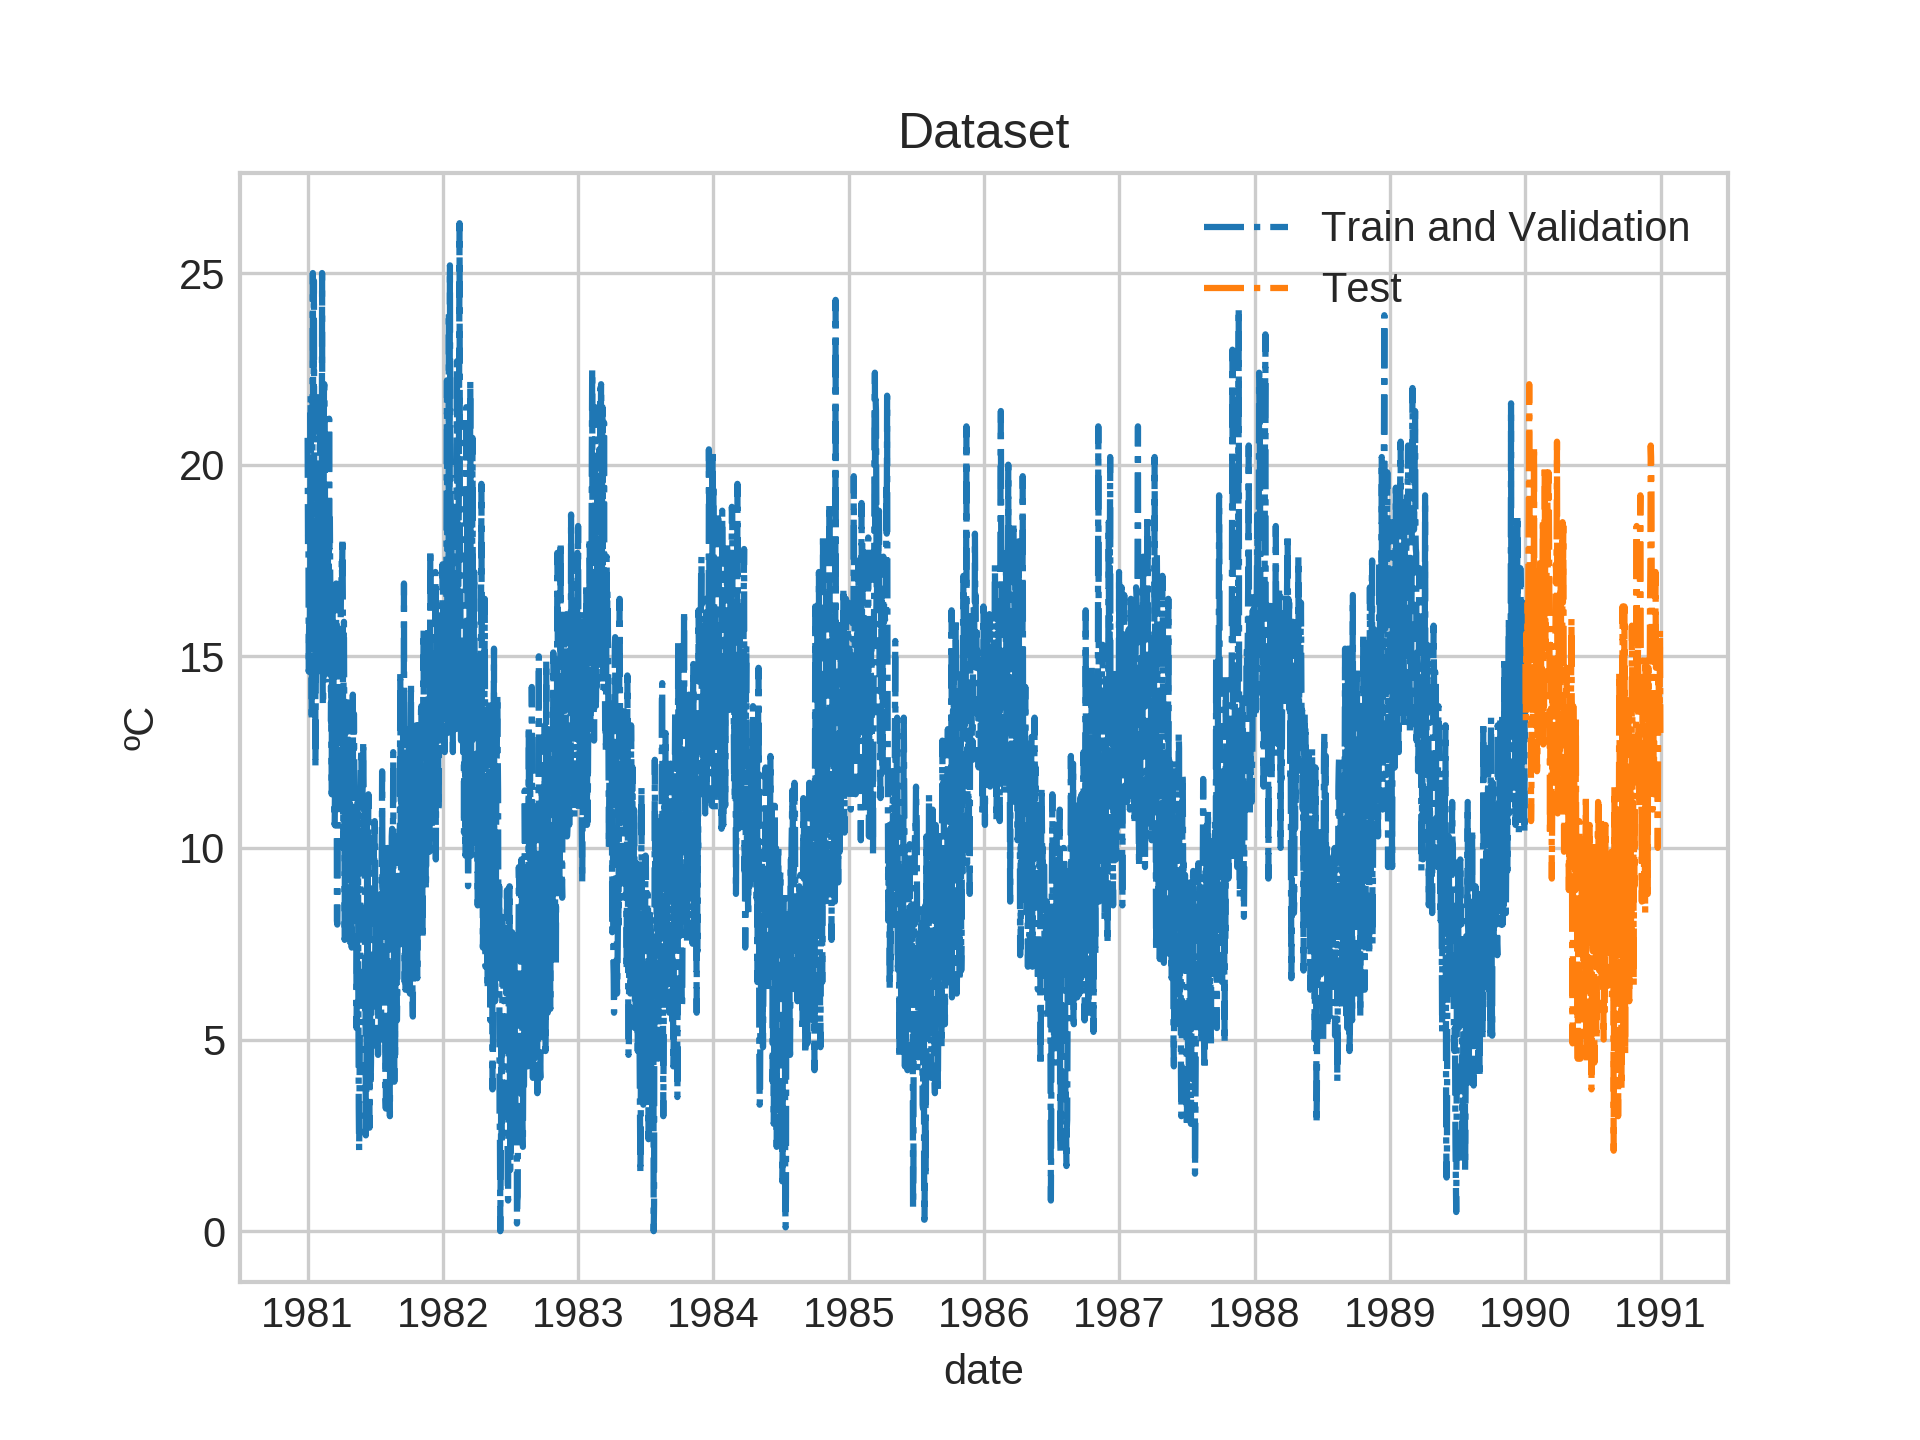
\includegraphics[width=\linewidth]{ex01/dataset.png}
        \caption{Temperatura mínima diária em Melbourne, Austrália, no período de 1981 a 1990.}
        \label{fig:dataset}
    \end{figure}
    
    Medidas de temperatura que não possuem amostras passadas suficientes serão descartadas, ou seja,
    a primeira amostra utilizada do \textit{dataset} será deslocada em $K + 1$, sendo $K$ os atrasos.
    \subsection[]{Exercício 01}
    O valor ótimo de atrasos a serem incluídos no vetor de entrada do preditor está condicionado
    ao resultado da validação do modelo para cada um dos $K$ atrasos, para $0\leqslant K \leqslant  30$.
    É aplicada a técnica de validação cruzada \textit{k-fold}, sendo $k$ o número de partes, $folds$.

    O número de \textit{folds} utilizado na validação do modelo foi definido como $k=10$ por ser um valor
    típico e separar para validação \textit{datasets} de comprimento próximo ao número de dias no ano. 
    
    Nota-se que a quantidade de atrasos (atributos) afeta o desempenho do modelo
    porém não possui uma relação linear com o RMSE da estimação \prettyref{fig:ex1_kfold_rmse}. Ganhos consideráveis
    são obtidos até certos valores de $K$.
    \begin{figure}[H]
        \centering
        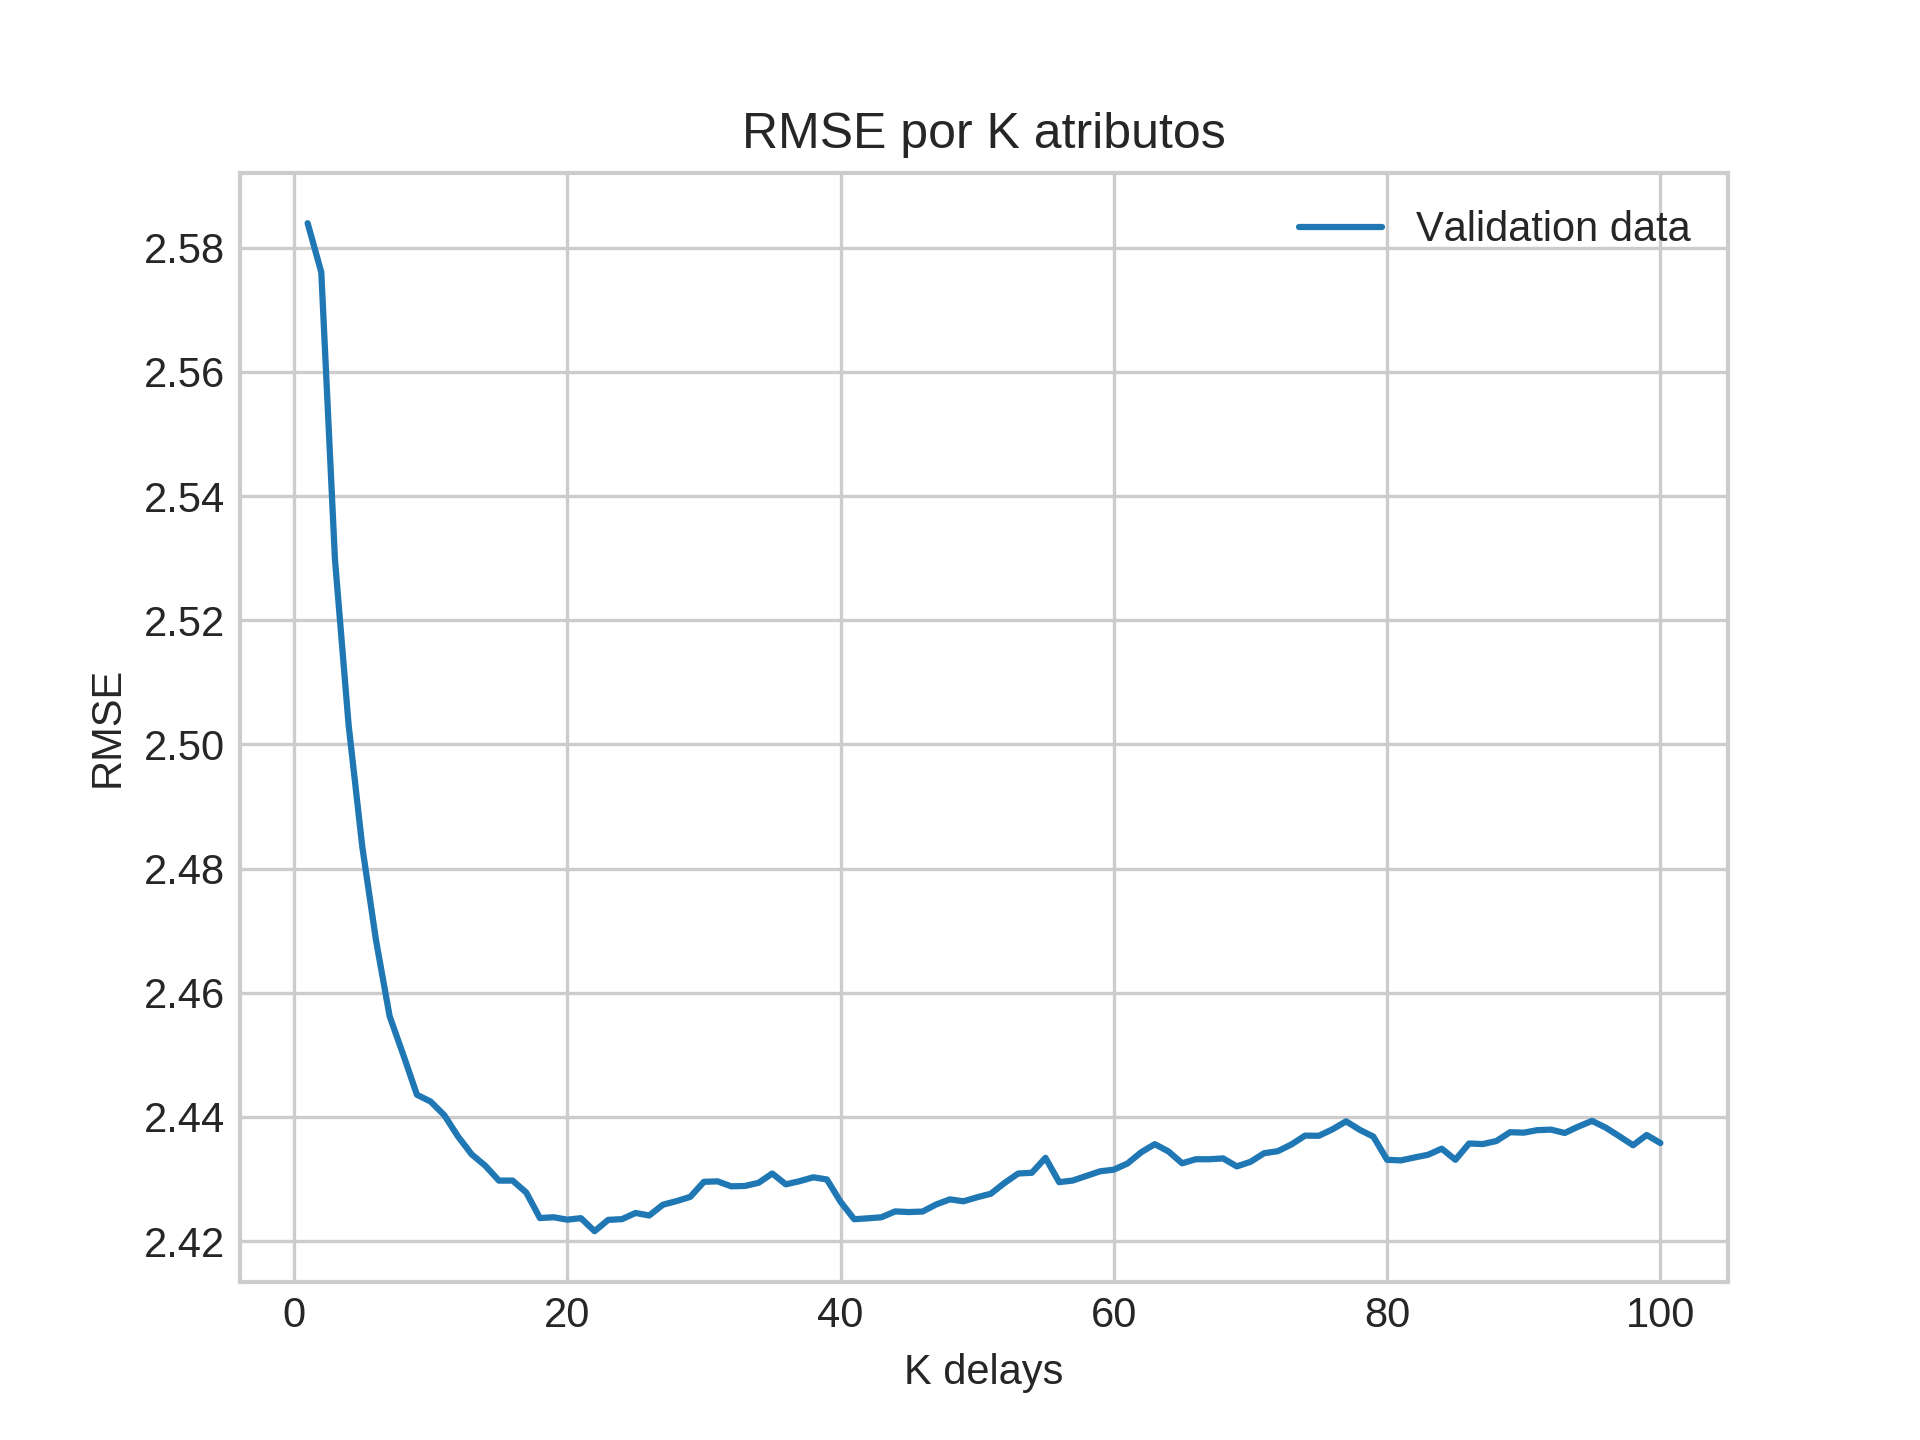
\includegraphics[width=\linewidth]{ex01/folds.png}
        \caption{Exercício 01: RMSE com validação cruzada \textit{10-folds} para $K$ \textit{delays}.}
        \label{fig:ex1_kfold_rmse}
    \end{figure}
    O número de atrasos $K=22$ apesentou $RMSE=2.4215989698821407$, o menor erro quadrático médio durante a validação dos modelos.
    Definido o número de atributos $K=22$, um novo modelo é calculado utilizando todos os dados (treinamento e validação).
    \begin{align*}
w=[ &0.60851412, 0.58768129, -0.08816496, 0.05312793, 0.03412434, 0.04066411, \\
    &0.028874  , 0.04560297,  0.01880947, 0.0336419,  0.00261787, 0.00780726, \\
    &0.01769519, 0.02374471,  0.00350507,  0.02043056,0.01260365, 0.0110618,  \\
    & 0.04655714, -0.00340386,  0.02787026,  0.01283307,  0.00674837]^T
    \end{align*}
    Uma vez obtido o vetor de pesos $w$ do preditor, o \textit{dataset} de testes é utilizado para
    sua avaliação final. A figura \prettyref{fig:ex1_model_comp} apresentas as saídas desejadas e as estimadas pelo modelo.

    Do teste realizado, foram obtidos erros de estimação \prettyref{fig:ex1_kfold_rmse} com as seguintes características:
    \begin{align}
       \sigma^2&=2.0928243101998594\\
       \sigma&=1.7478639423536222\\
       \mu&=1.4466597078096353\\
       min(RMSE)&=0.0015856919462313712\\
       max(RMSE)&=7.12356630491203 
   \end{align}

   \begin{figure}[H]
        \centering
        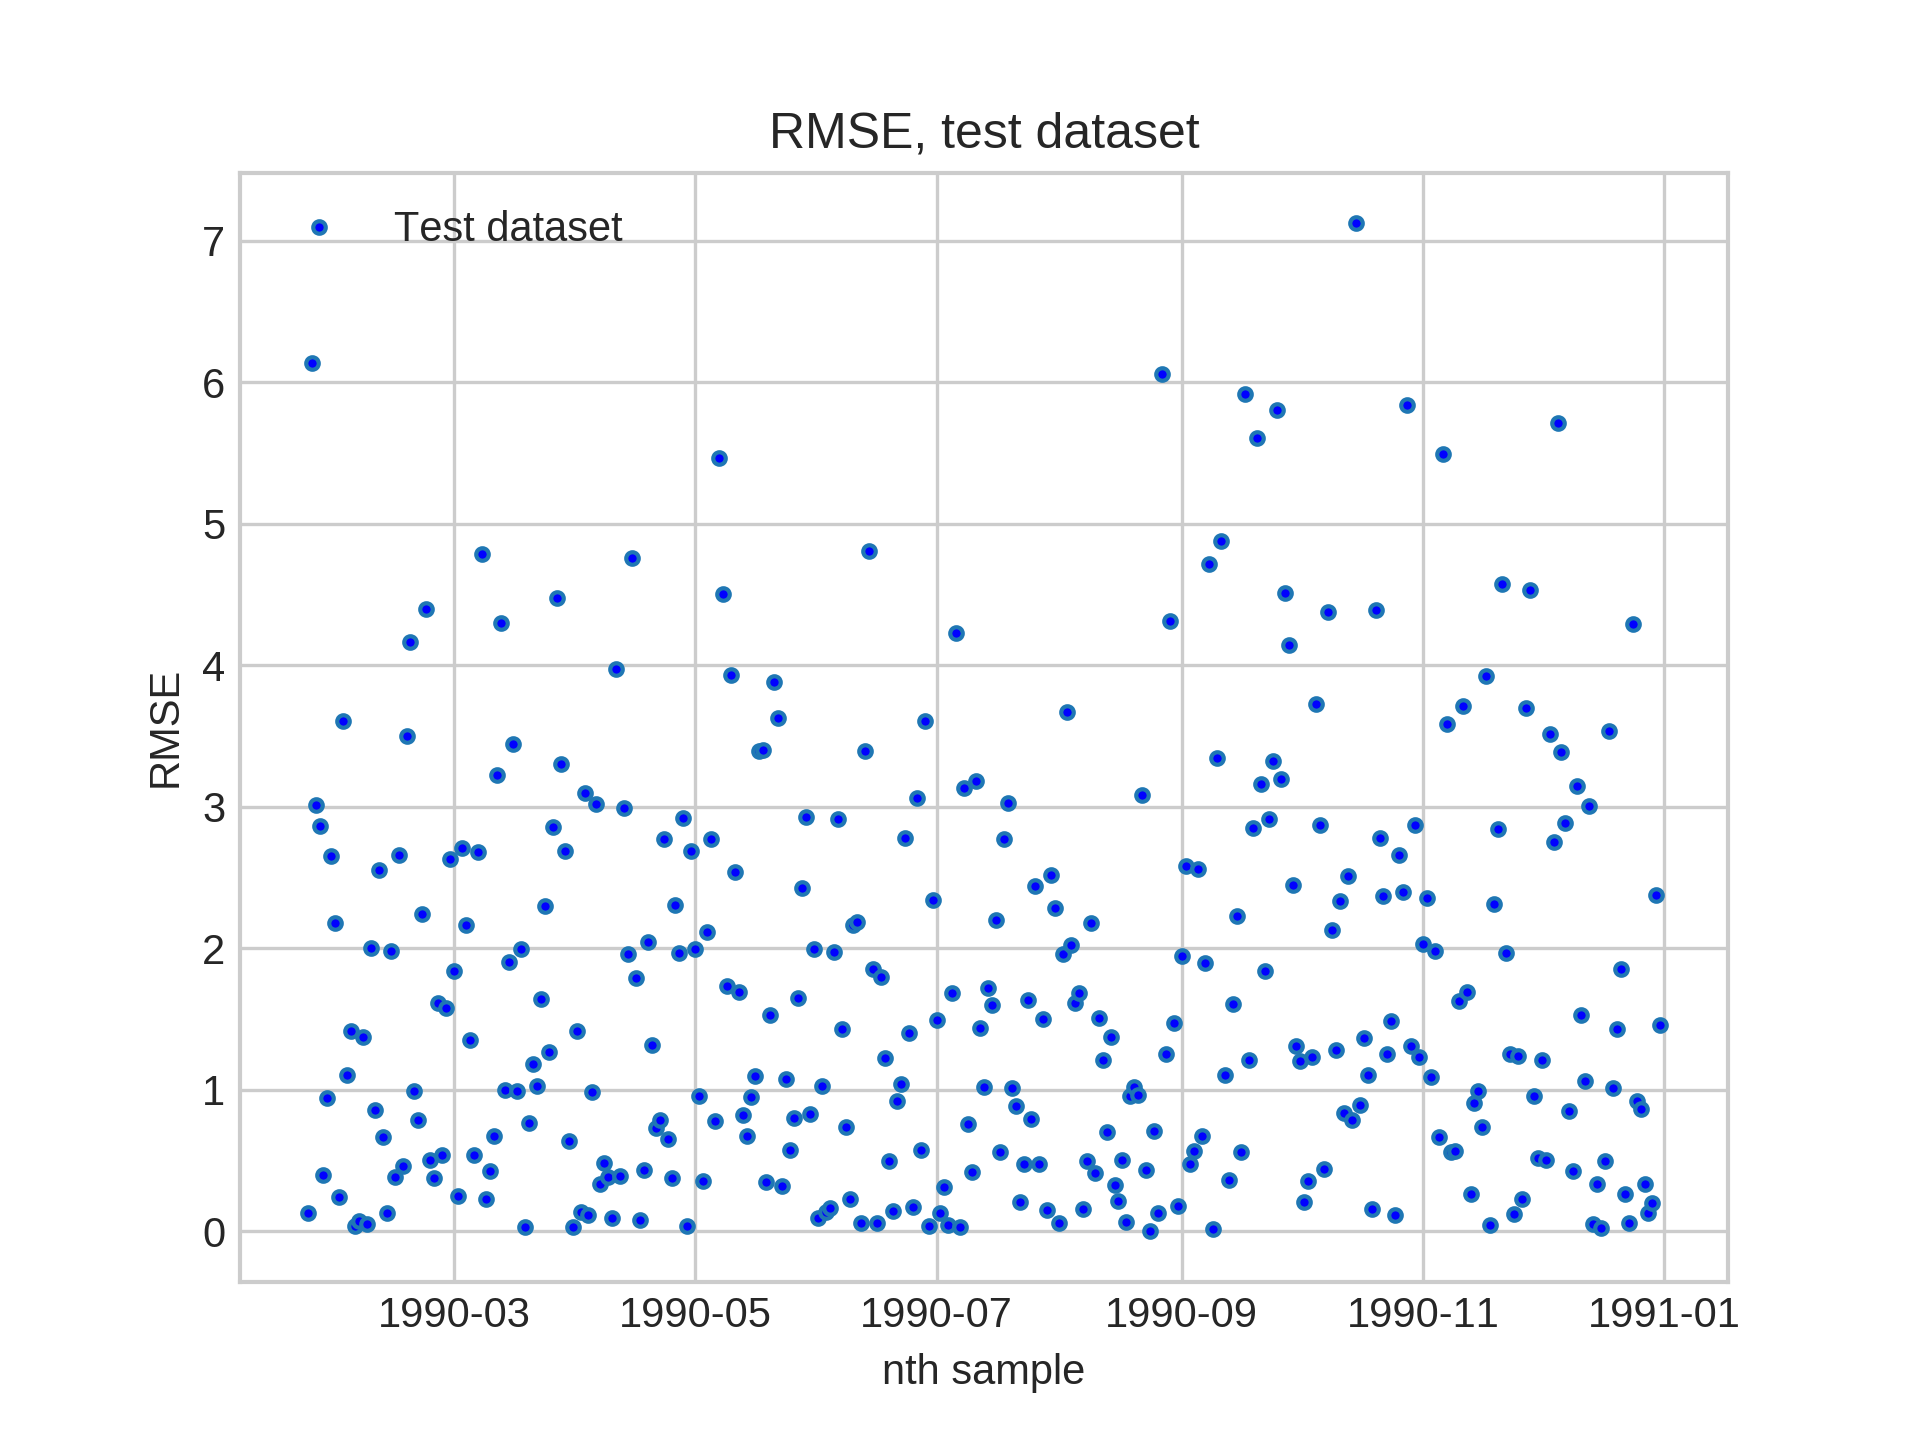
\includegraphics[width=\linewidth]{ex01/model.png}
        \caption{Exercício 01: RMSE do \textit{dataset} de teste para o modelo escolhido.}
        \label{fig:ex1_kfold_rmse}
    \end{figure}
    As estimações de temperatura e os valores esperados para o \textit{dataset} de teste são
    mostrados na figura \prettyref{fig:ex1_model_comp}.
    \begin{figure}[H]
        \centering
        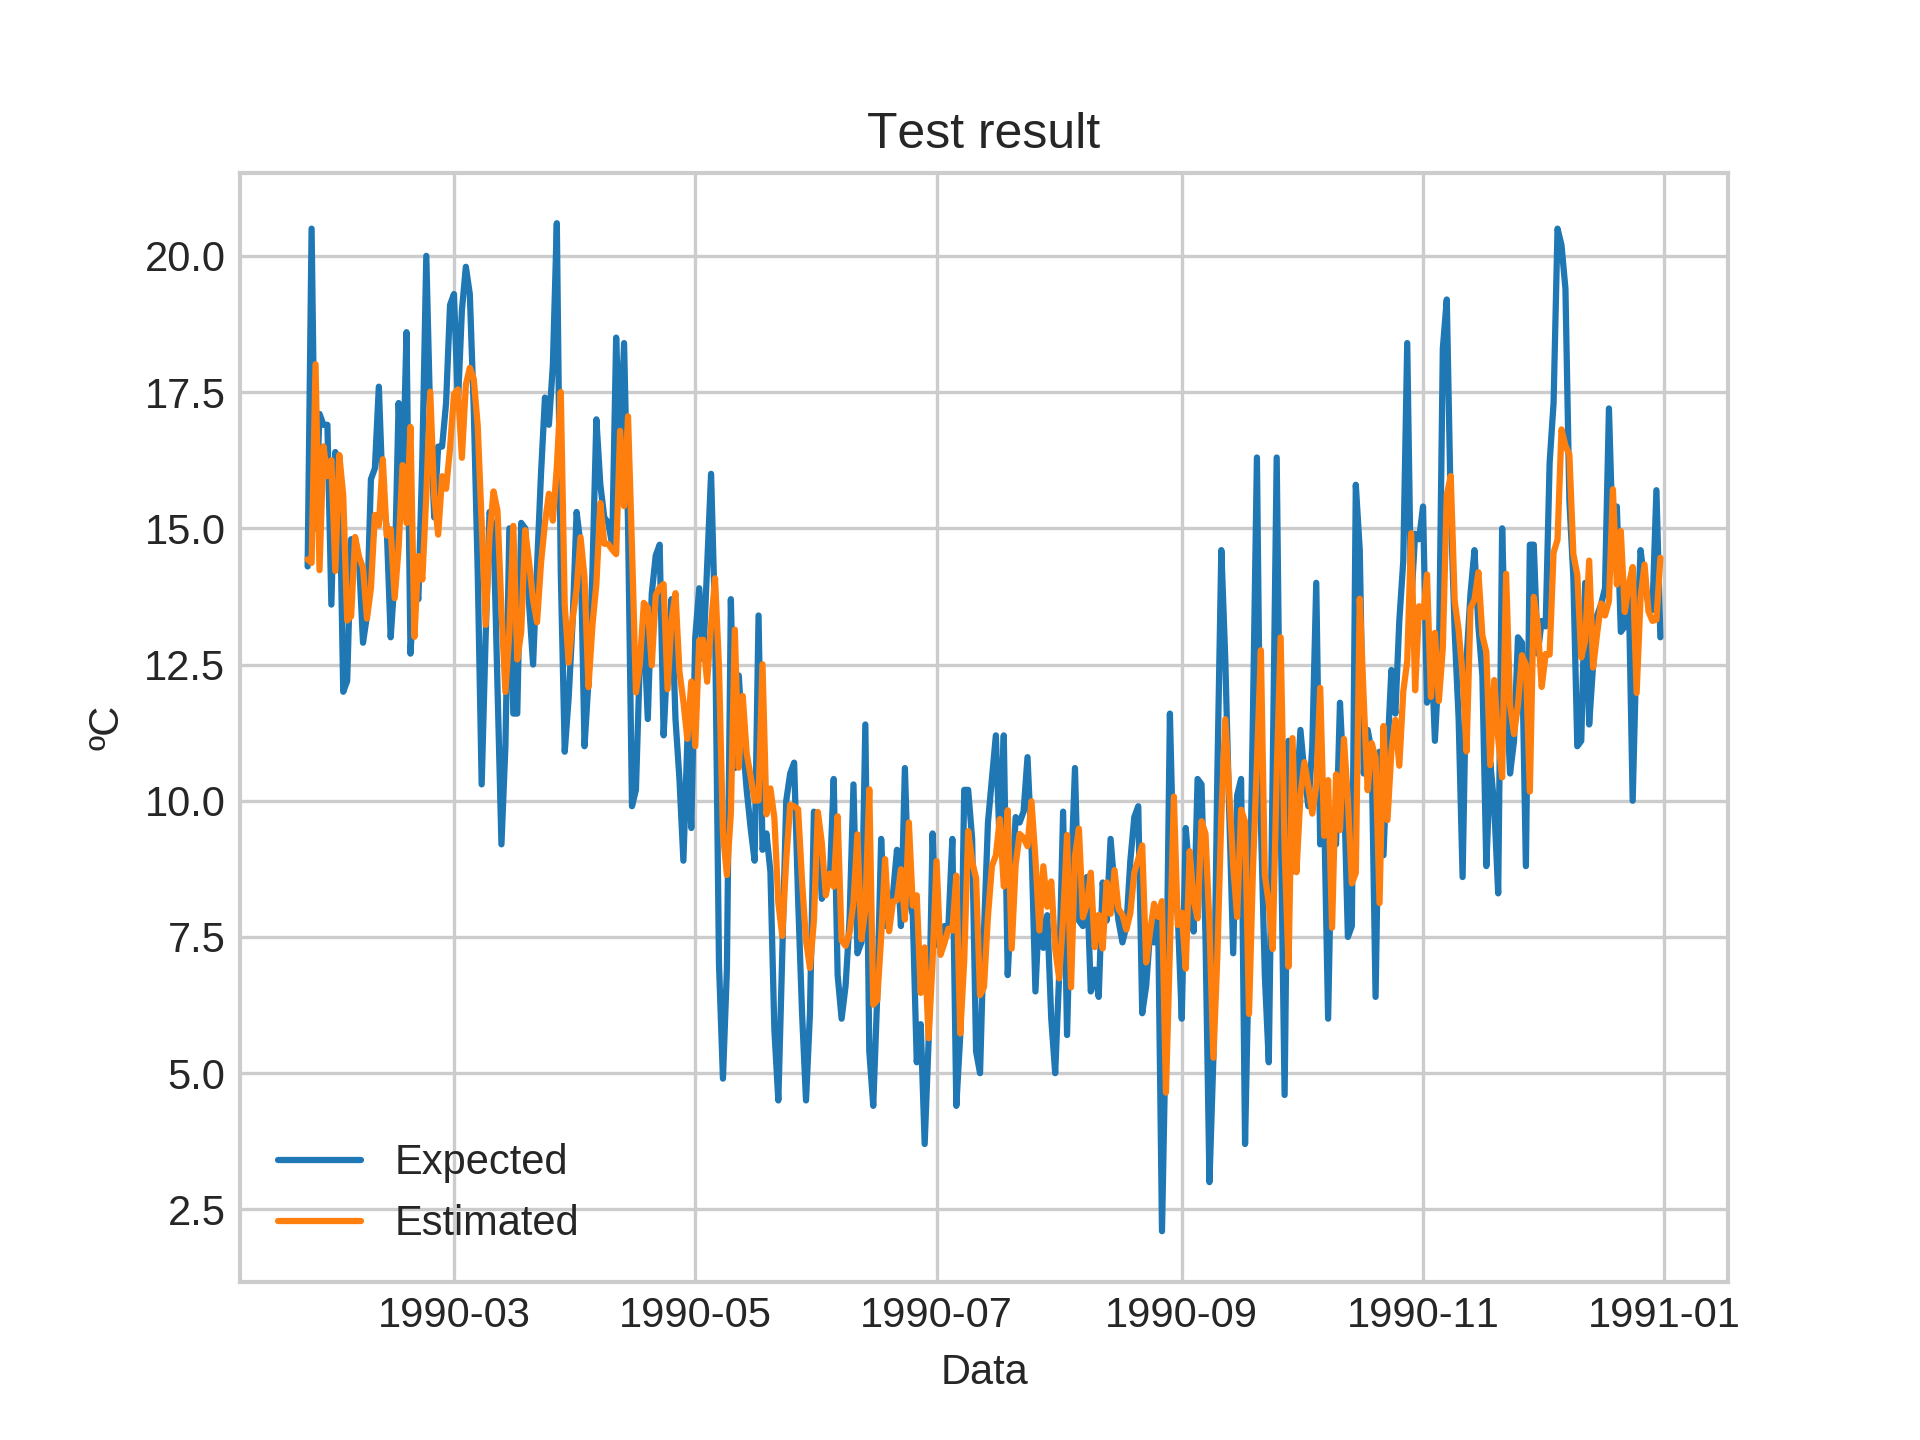
\includegraphics[width=\linewidth]{ex01/model_comp.png}
        \caption{Exercício 01: Estimação do modelo para o \textit{dataset} de teste e o valor esperado.}
        \label{fig:ex1_model_comp}
    \end{figure}
    
    \newpage
    \subsection[]{Exercício 02}
    São mostrados na figura \prettyref{fig:ex2_TRMSE} os erros de estimação dado o número de atributos.
    É mostrada a estimação do modelo com parâmetro de regularização $\lambda$ que de menor RMSE na validação cruzada.
    Para cada $T$ atributos é utilizado um $\lambda$ específico obtido através do
    método da Seção Áurea com critério de parada de $0.001\%$ na variação do RMSE.
    Foram utilizados na geração dos atributos $T$,
    pesos obtidos a partir de uma distribuição uniforme na faixa $]-1,1[$
    \begin{figure}[H]
        \centering
        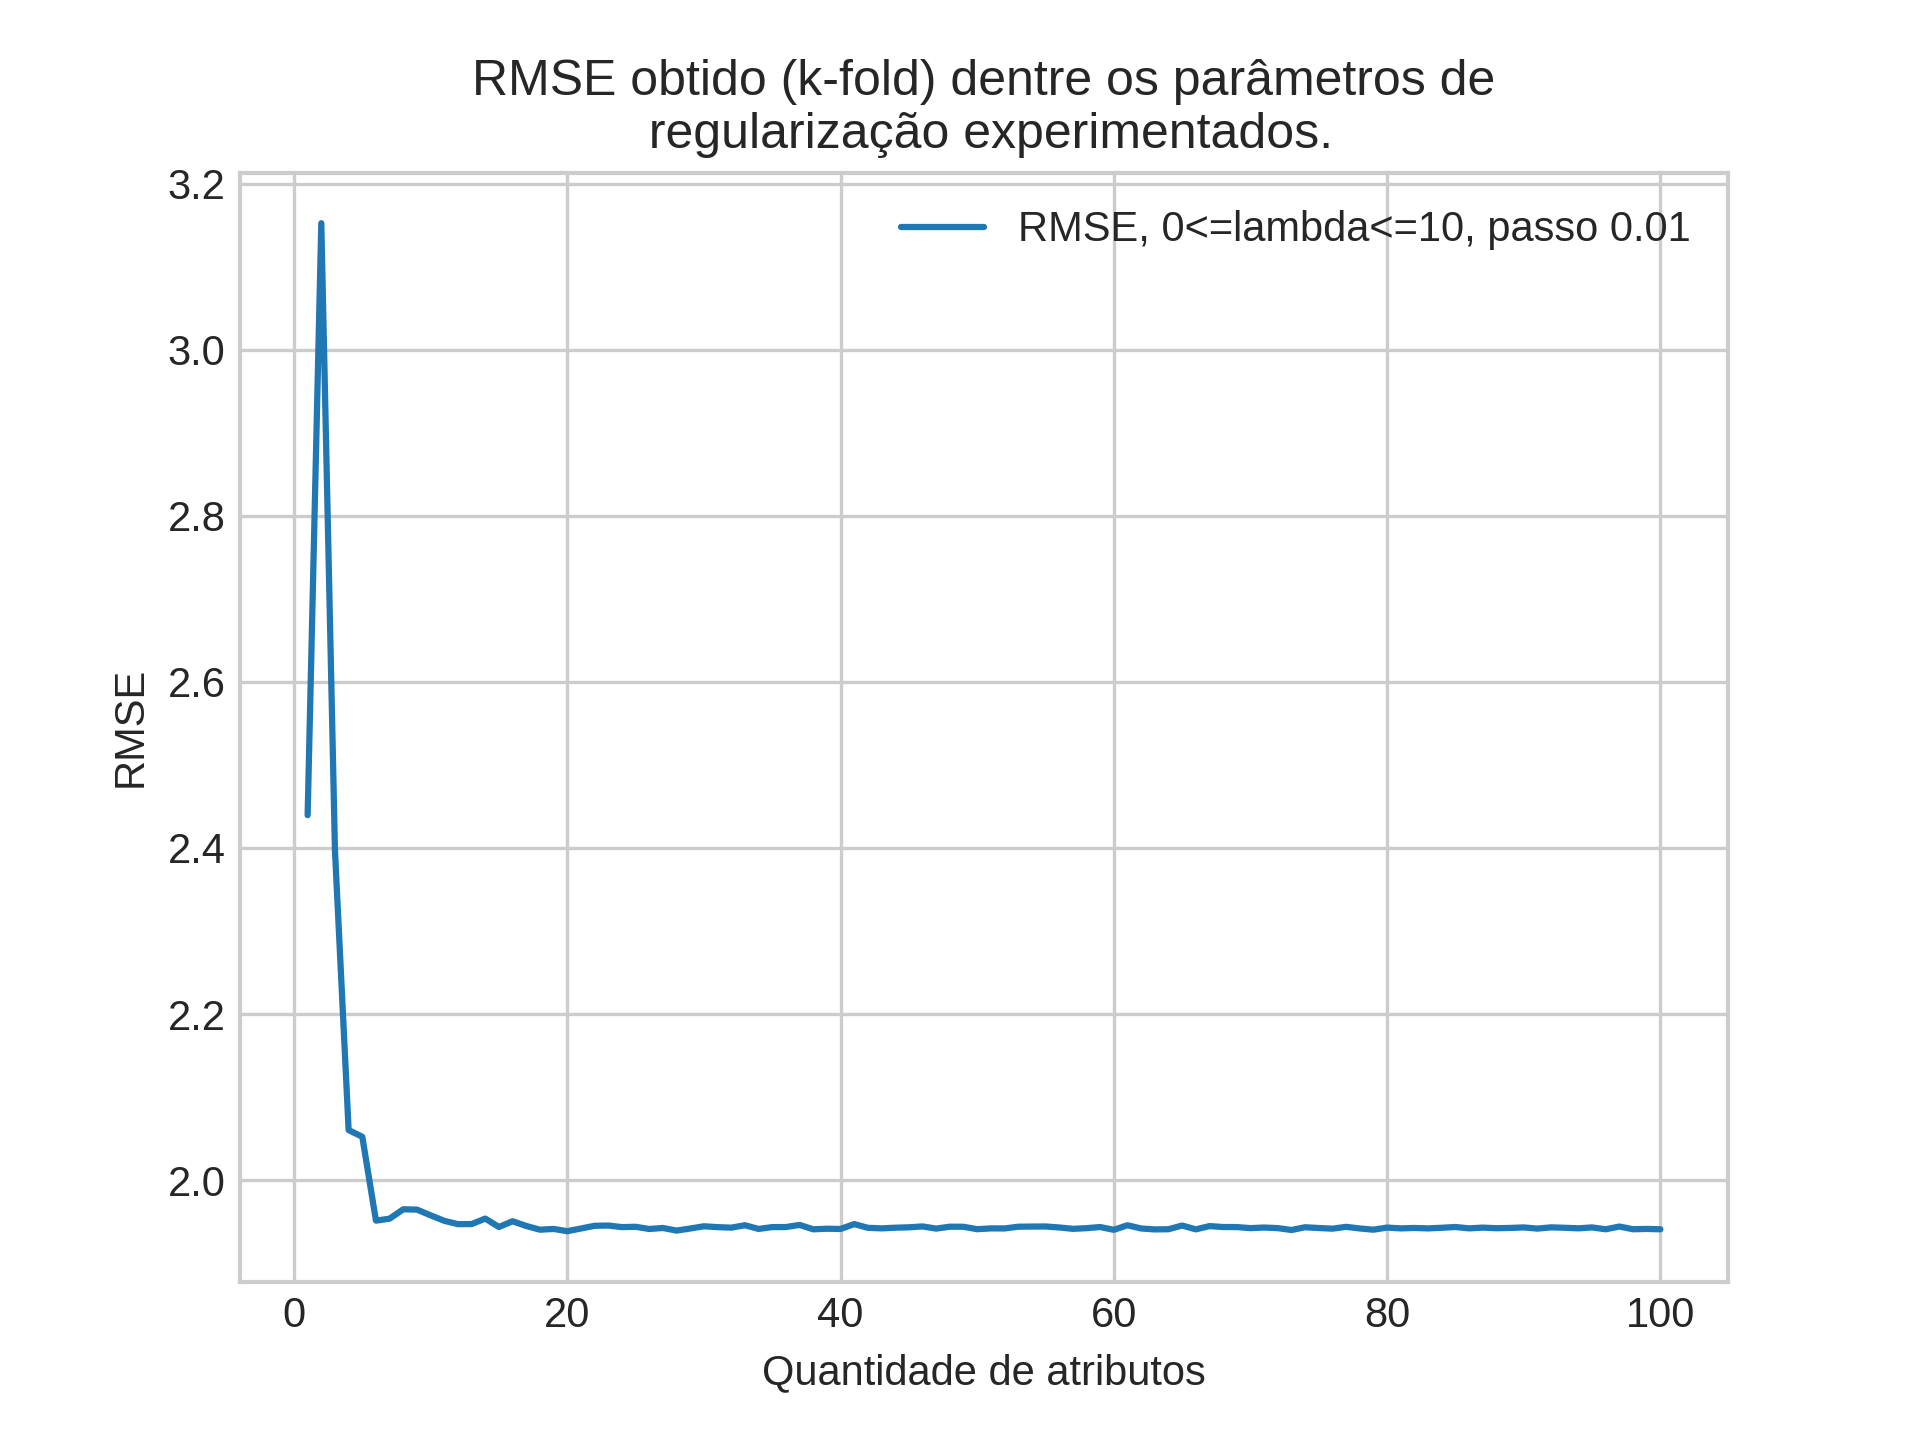
\includegraphics[width=\linewidth]{ex02/TsMeans.png}
        \caption{Exercício 02: RMSE em função do número de atributos $T$.}
        \label{fig:ex2_TRMSE}
    \end{figure}
    
    O melhor parâmetro de regularização $\lambda$, para cada valor de $T$ é apresentado na figura \prettyref{fig:ex2_Tlamb}.
    \begin{figure}[H]
        \centering
        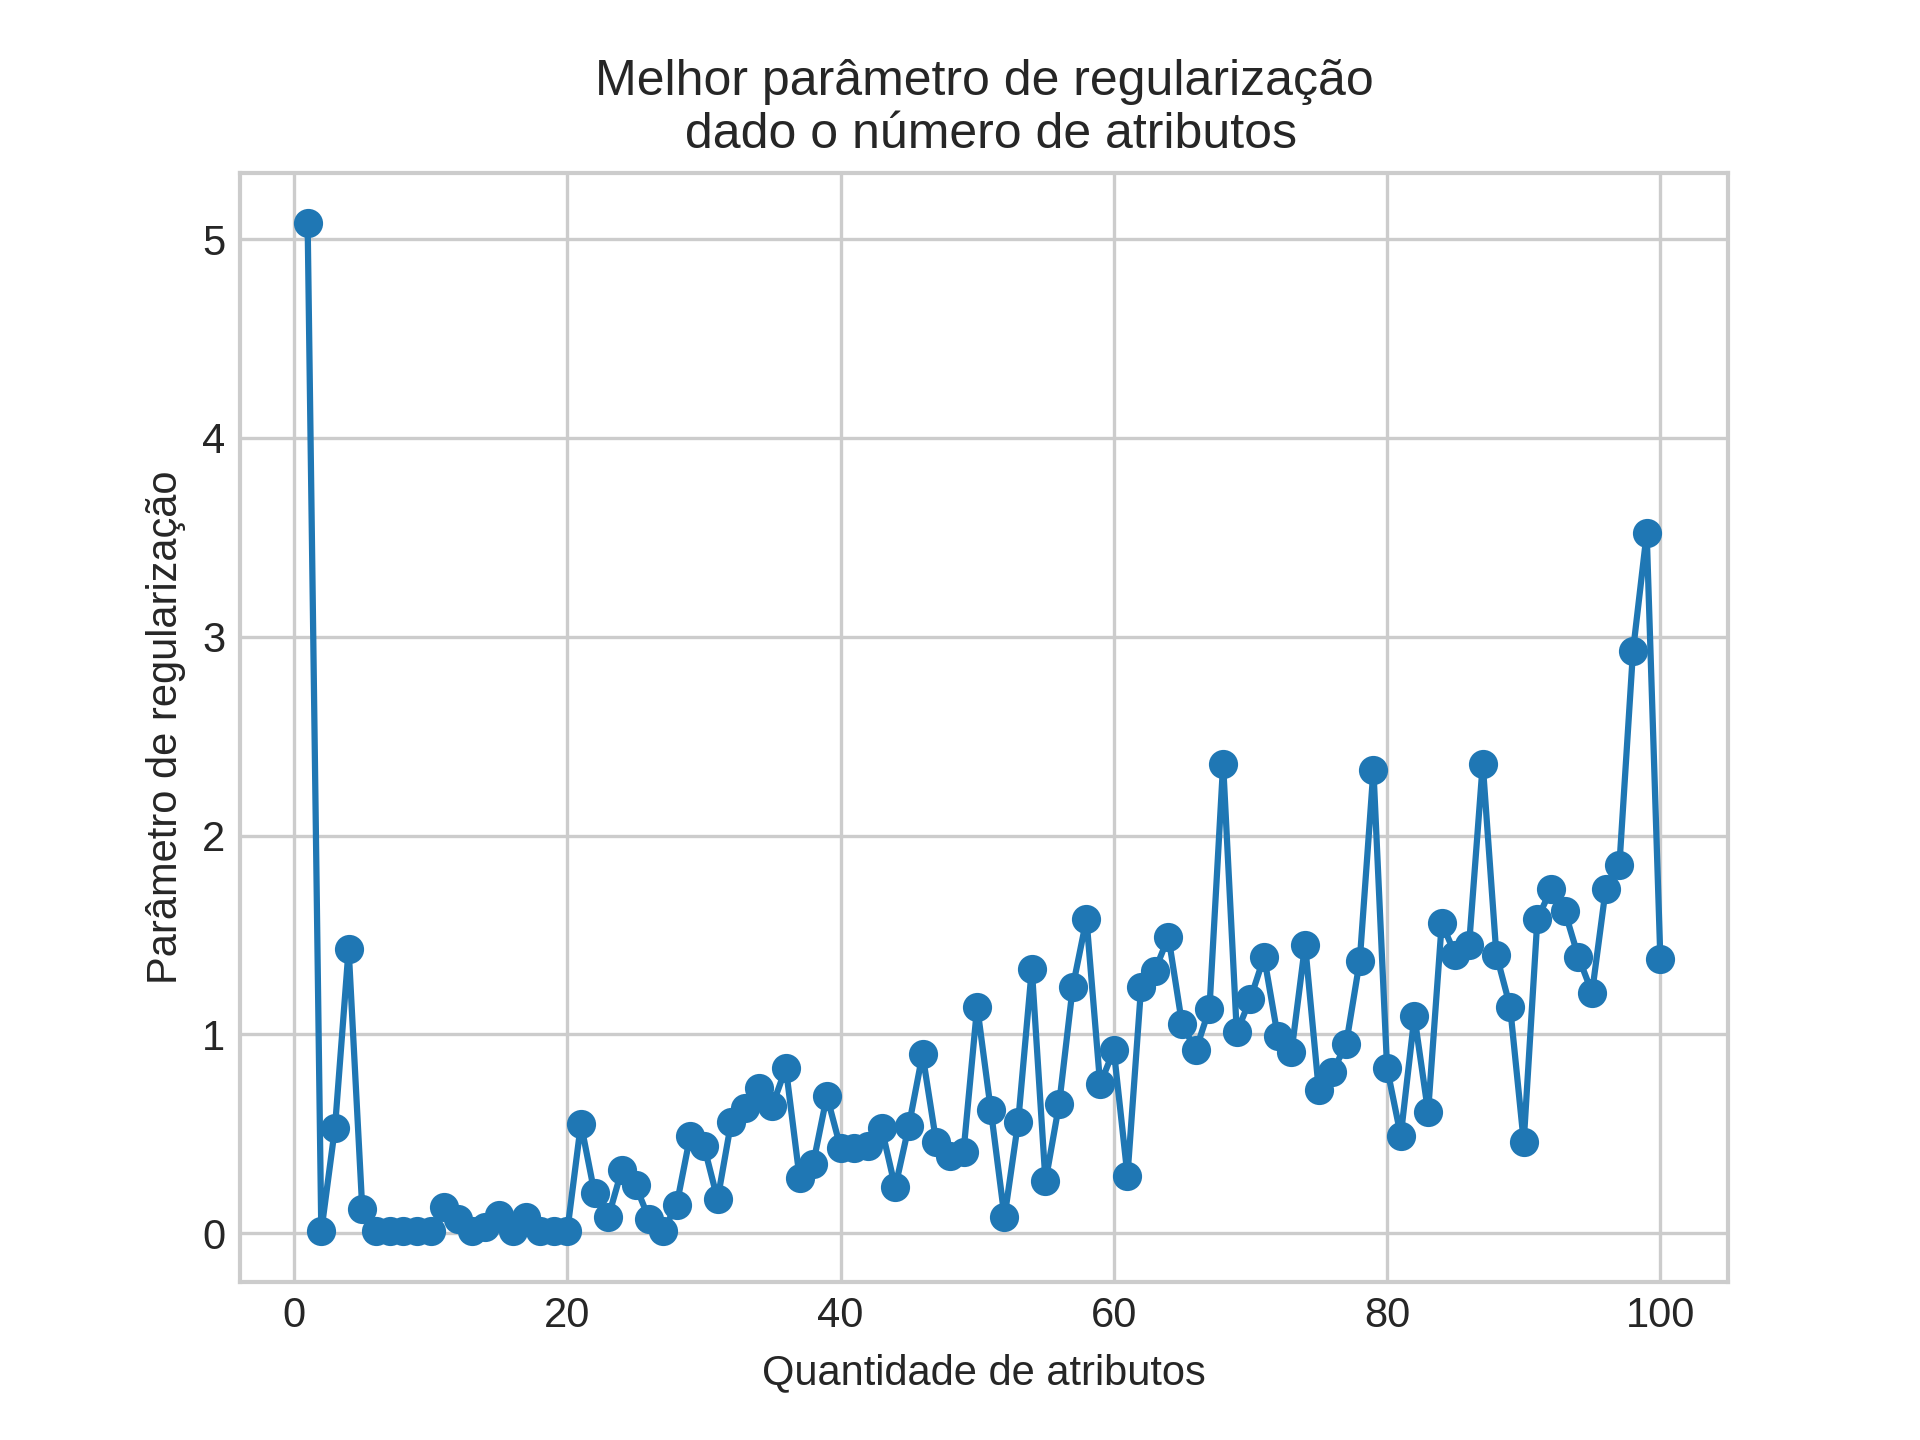
\includegraphics[width=\linewidth]{ex02/Tslambs.png}
        \caption{Exercício 02: Melhor $\lambda$ para dados $T$ atributos.}
        \label{fig:ex2_Tlamb}
    \end{figure}
 
    O melhor modelo obtido possui $T=27$ atributos com o parâmetro de regularização $\lambda=0.05952670961077918$.
    No \textit{dataset} de testes foram obtidos os seguintes resultados referentes ao RMSE da predição \prettyref{fig:ex2_rmse}:
    \begin{align}
        \sigma^2&=2.14764650270121\\
        \sigma&=1.8063483044164936\\
        \mu&=1.4654850741993963\\
        min(RMSE)&=0.003573731813188985\\
        max(RMSE)&=7.320990019087004\\
    \end{align}
    \begin{figure}[H]
        \centering
        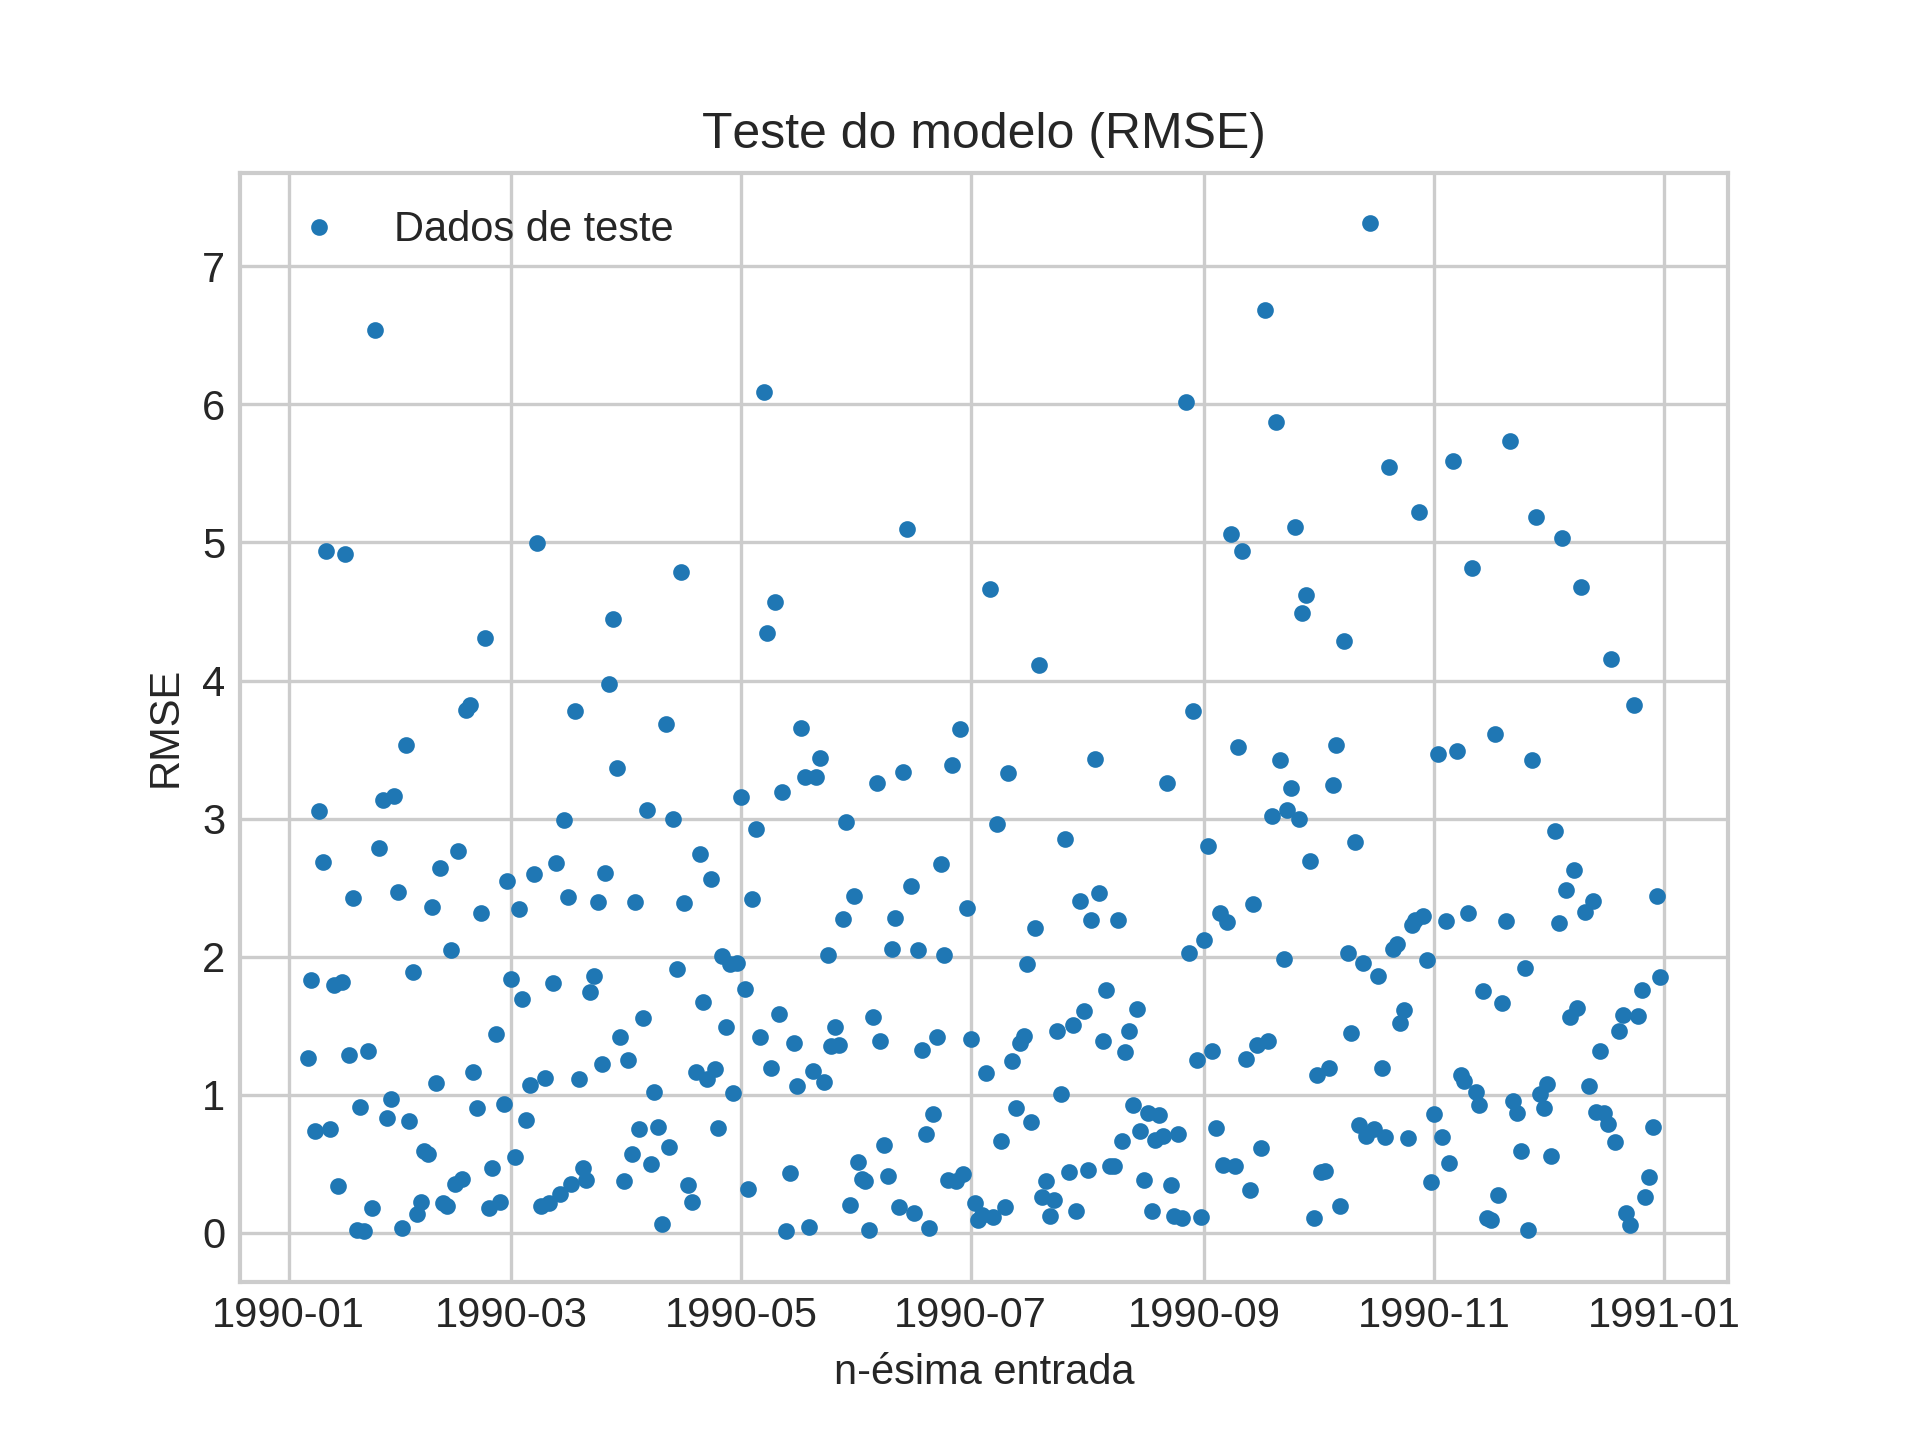
\includegraphics[width=\linewidth]{ex02/model_rmse.png}
        \caption{Exercício 02: RMSE do \textit{dataset} de teste para o modelo escolhido.}
        \label{fig:ex2_rmse}
    \end{figure}

    O gráfico dos resultados esperados do \textit{dataset} de testes e as estimações do modelo podem ser vistas na figura \prettyref{fig:ex2_comp}. 
    \begin{figure}[H]
        \centering
        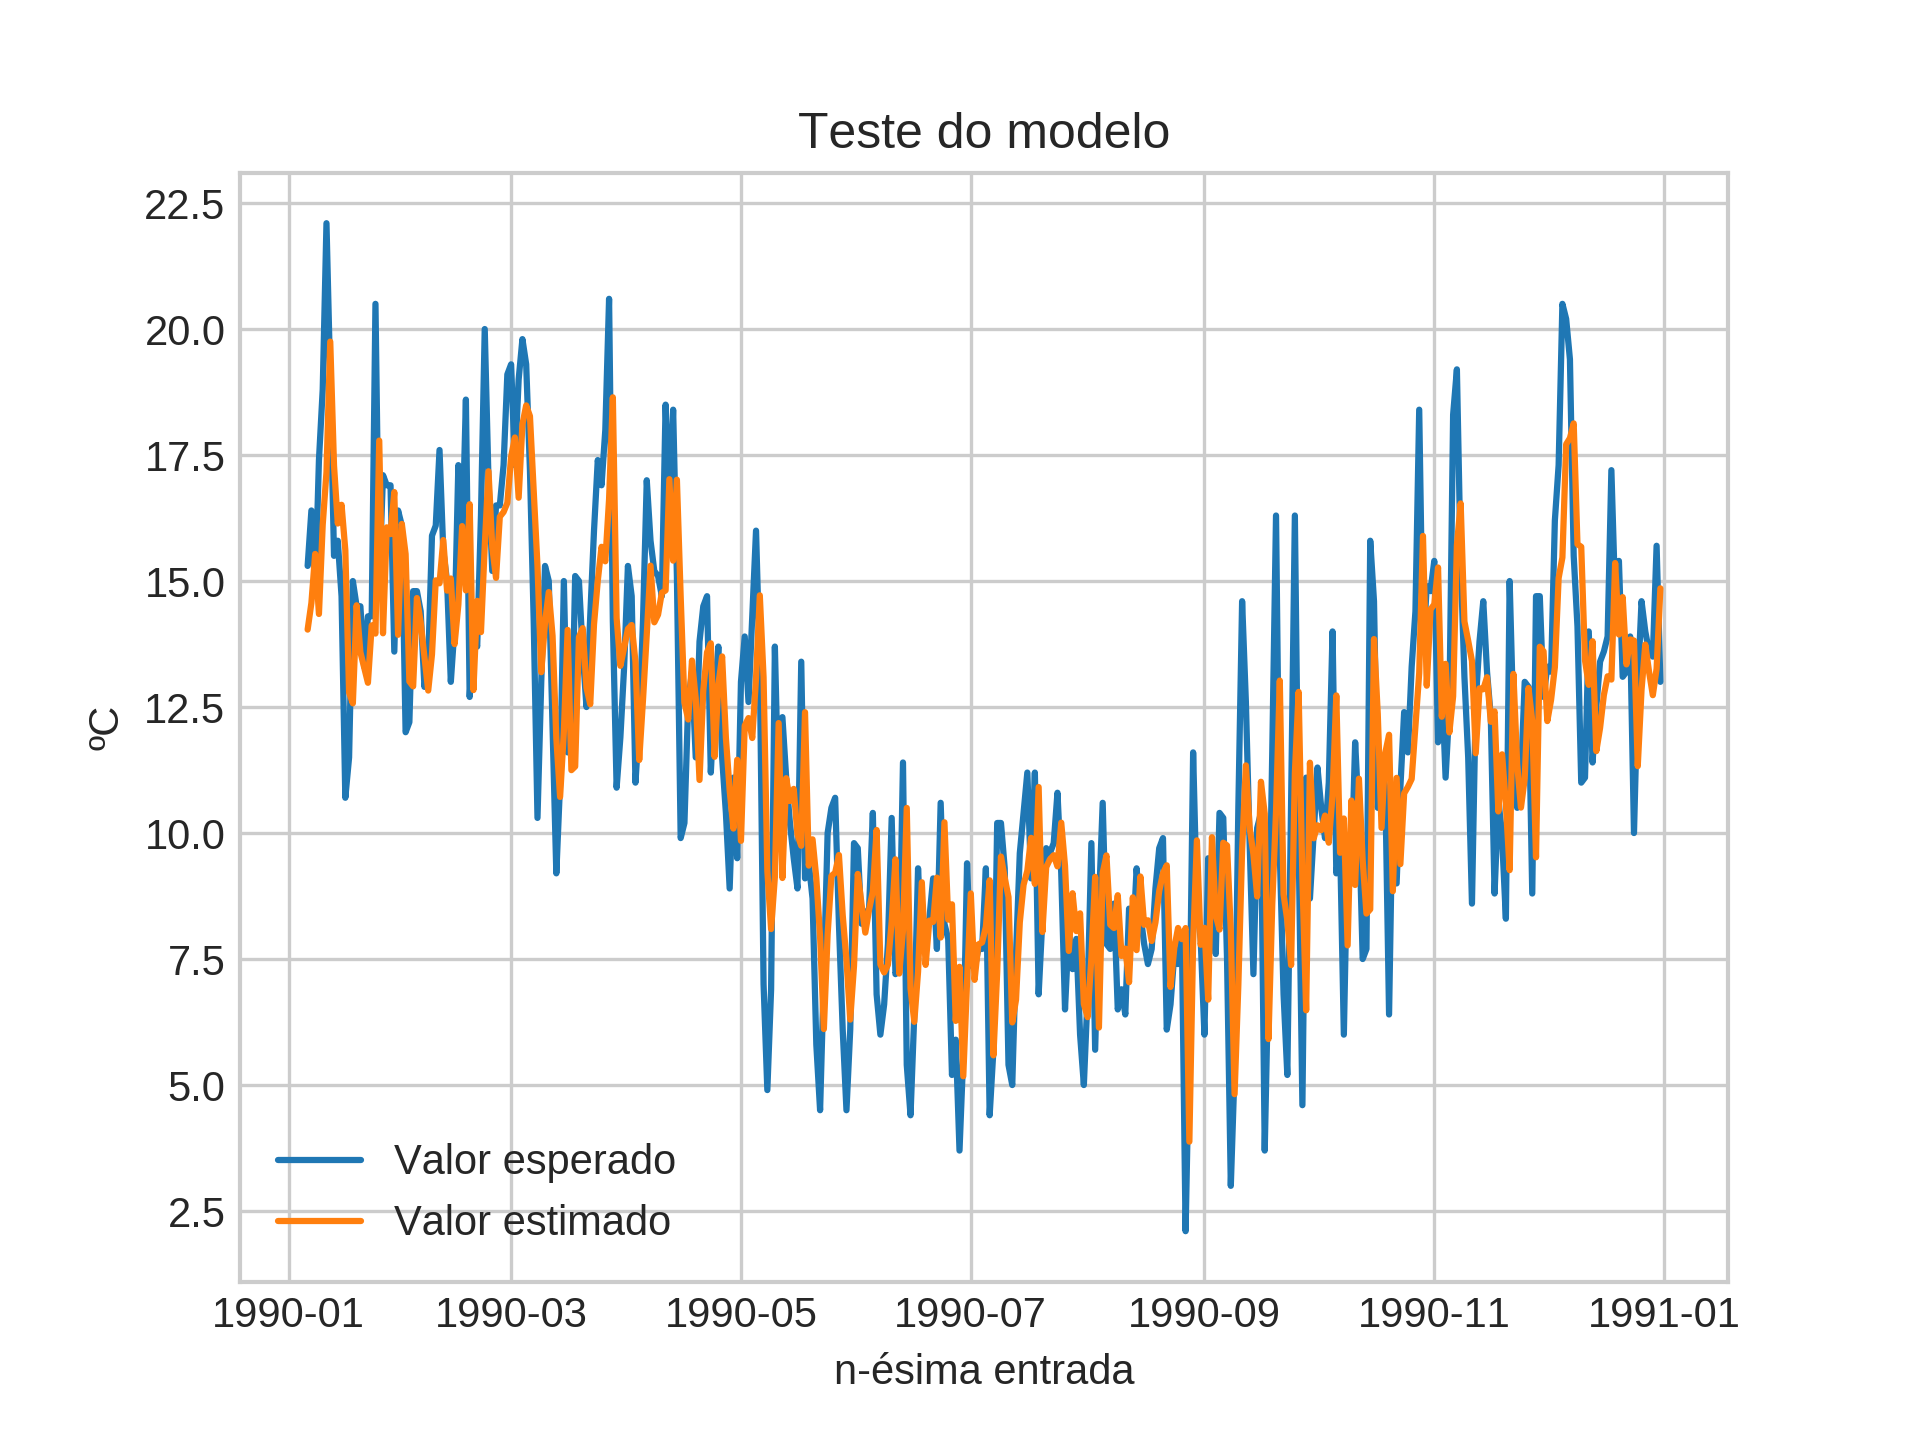
\includegraphics[width=\linewidth]{ex02/model_test.png}
        \caption{Exercício 02: Estimação do modelo para o \textit{dataset} de teste e o valor esperado.}
        \label{fig:ex2_comp}
    \end{figure}
\end{document}